\setcounter{section}{71}
\section{Определения сети, потока, величины потока, остаточной сети. Пример, почему нельзя обойтись без обратных рёбер.}
\par \textbf{Определение:} \textit{Сеть} - это $(G, s, t, c)$, где $G=(V, E)$ - ориентированный граф (без петель и кратных ребер), $s, t$ - различные вершины из $V$ ($s$ - исток (source), $t$ - сток (target)), $c: E \rightarrow \mathbb{Z}_+$ - пропускные способности (capacity) на каждом ребре.
\par \textbf{Определение:} $f: V \times V \rightarrow \mathbb{Z}$ называется \textit{потоком} в сети $G$, если выполняются следующие условия\begin{enumerate}
    \item $\forall u \forall v \: f(u,v) \leq c(u,v)$ (если $(u,v)\not\in E$, то $c(u,v)=0$)
    \item Сохранение потока (сколько втекло в вершину столько и вытечет): $\forall v \in V \setminus \{s, t\} \hookrightarrow \sum_{(u,v)\in E}f(u,v)=\sum_{(v,w)\in E} f(v,w)$
    \item Антисимметричность: $f(u,v)=-f(v,u)$
\end{enumerate}
\par \textbf{Определение:} \textit{Величиной потока} называется число $|f|=\sum_{v \in V} f(s, v)$
\par \textbf{Определение:} Пусть $G$ - сеть, $f$ - поток в ней. Тогда \textit{остаточной сетью} $G_f$ называется сеть с $c_f(u,v)=c(u,v)-f(u,v)$
\par \textbf{Пример:} Слева граф, справа - его остаточная сеть.
\begin{figure}[h]
\hfill
\hspace{-4ex} \begin{minipage}[h]{0.5\linewidth}
\center{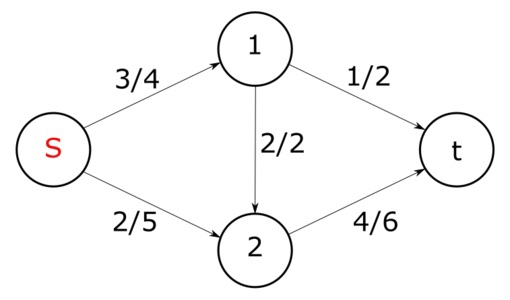
\includegraphics[width=1\linewidth]{images/72-85_graph.jpg}}
\end{minipage}
\hfill
\hspace{-4ex} \begin{minipage}[h]{0.5\linewidth}
\center{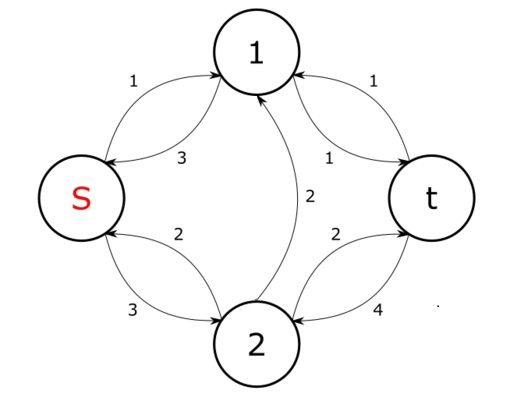
\includegraphics[width=1\linewidth]{images/72-85_remain_net.jpg}}
\end{minipage}

\end{figure}
\begin{figure}[h]
\hfill
\hspace{-4ex} \begin{minipage}[h]{0.5\linewidth}
\par \textbf{Пример:} Зачем нужны отрицательные ребра? Ответ: чтобы отменять действия, которые нам не нравятся
\end{minipage}
% \hfill
\hspace{-4ex} \begin{minipage}[h]{0.5\linewidth}
\center{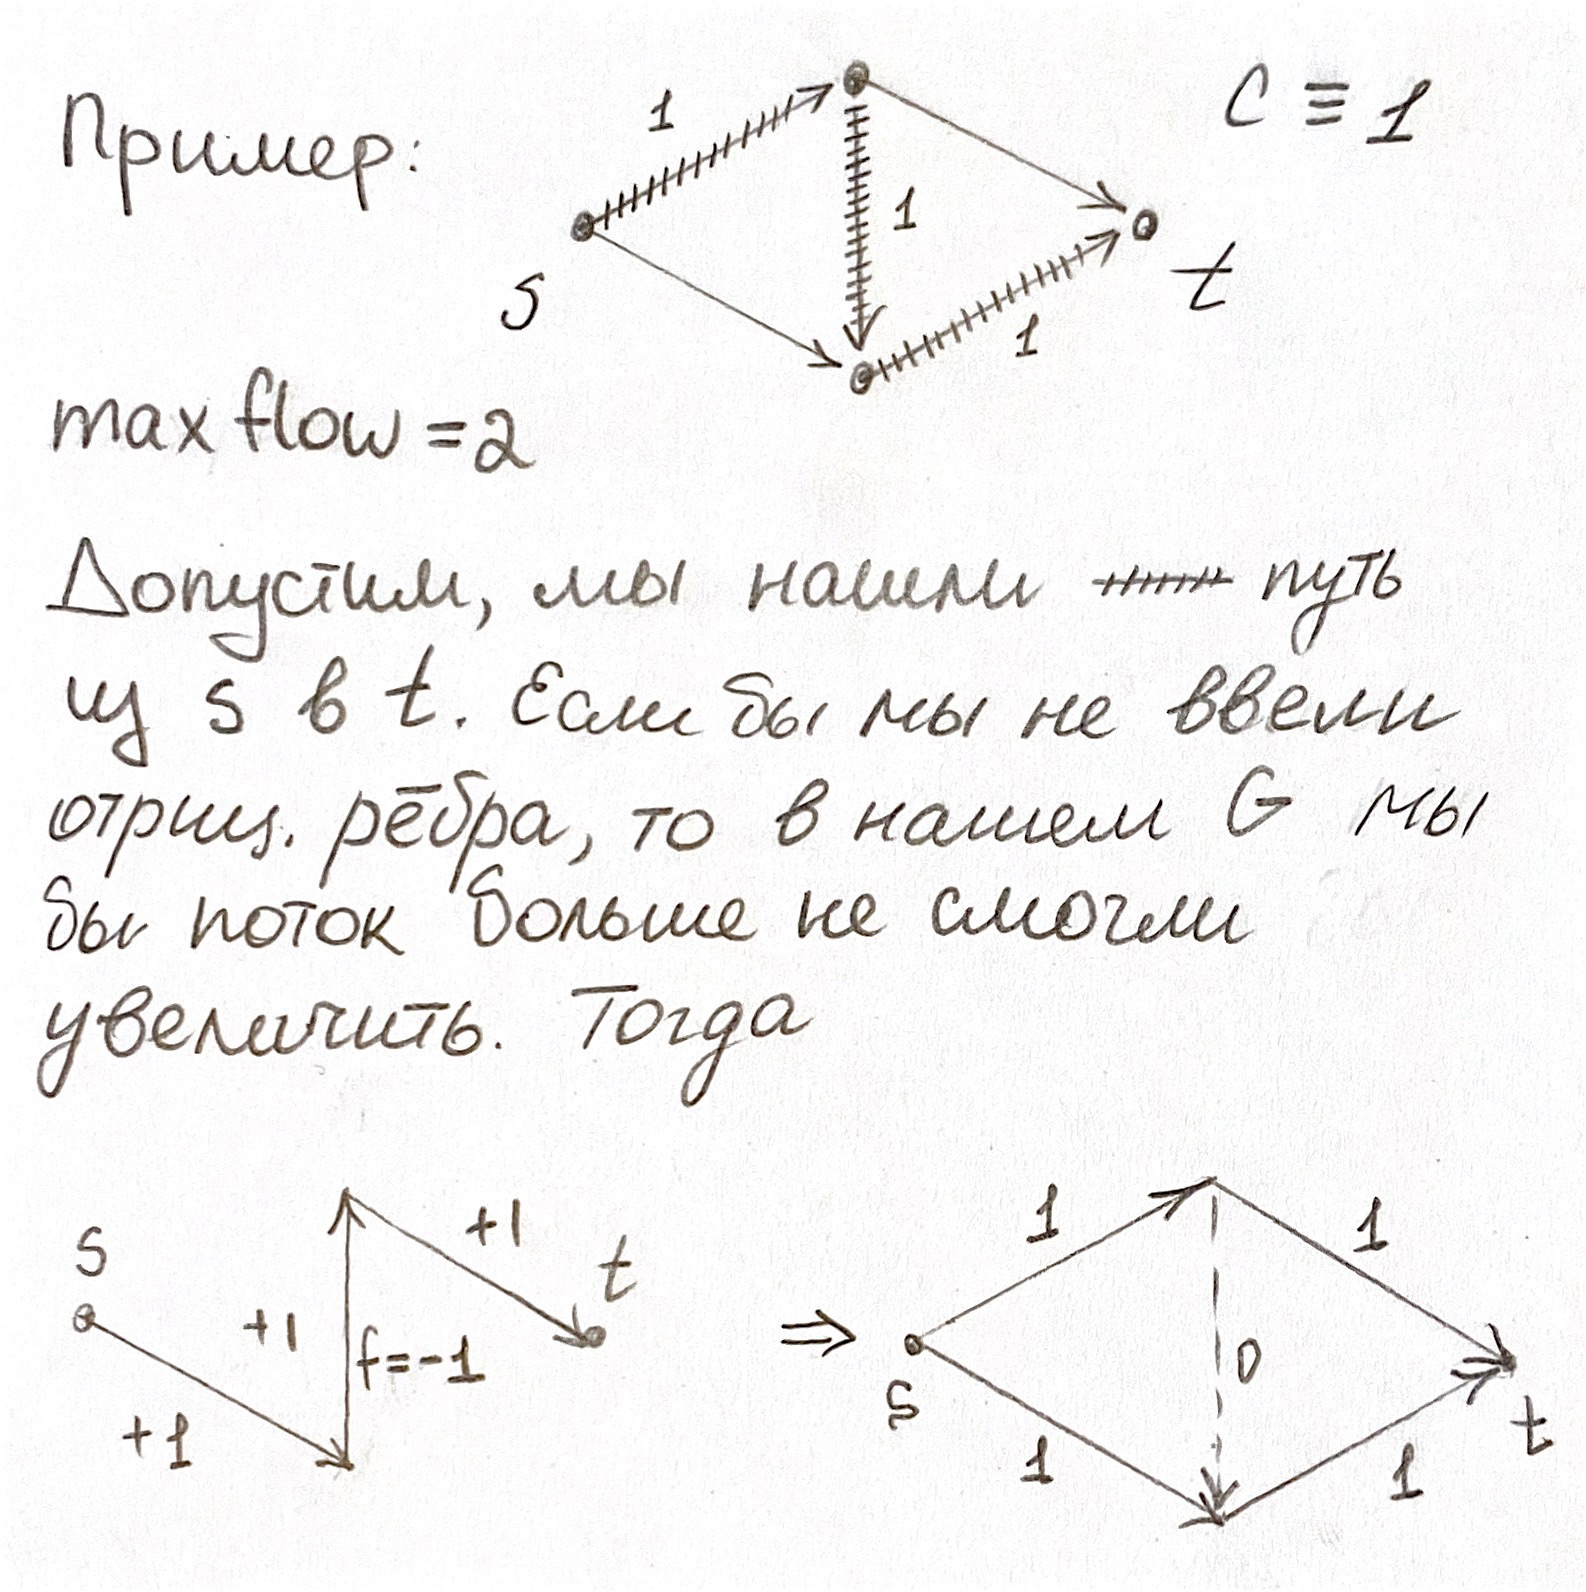
\includegraphics[scale=0.1]{images/72-85_reverse_edges.jpg}}
\end{minipage}

\end{figure}
\setcounter{section}{72}
\section{Определения разреза, величины разреза, величины потока через разрез. Лемма о равенстве величины потока и величины потока через разрез.}
\par \textbf{Определение:} $G$ - сеть. $(S,T)$ - \textit{разрез}, если $s \in S, \: t \in T, \: S \sqcup T=V$. 
$$c(S,T)=\sum_{u \in s, v\in T} c(u,v) \text{ - величина разреза}$$
$$f(S,T)=\sum_{u \in s, v\in T} f(u,v) \text{ - величина потока через разрез}$$
\par \textbf{Лемма:} $\forall (S,T)$ - разрез выполнено $f(S, T)=|f|$
\par $\blacktriangle$ Доказательство индукцией по величине $S$
\begin{enumerate}
    \item $S=\{s\} \Rightarrow (\{s\}, V \setminus \{s\})$ - разрез
    $$f(\{s\}, V \setminus \{s\})=\sum_{v \in V \setminus \{s\}}f(s,v)=|f| \text{ (так как $f(s,s)=0$)}$$
    \item $S=\{s, v_1, \ldots, v_{i+1}\}$. Пусть $U=\{s, v_1, \ldots, v_{i}\}$ и $f(U, V \setminus U)=|f|$. Тогда при добавлении $v_{i+1}$ часть ребер перестанут вносить вклад в величину разреза (из $u \in U$ в $v_{i+1}$), а часть - начнут (из $v_{i+1}$ в $w \in V \setminus U \Leftrightarrow w \not\in U$). Тогда
    $$f(S, V\setminus S)=f(U, V \setminus U)-\sum_{u \in U} f(u, v_{i+1})+\sum_{w \not\in U} f(v_{i+1}, w)=|f|-\sum_{u \in U} f(u, v_{i+1})+\sum_{w \not\in U} f(v_{i+1}, w)$$
    \par Покажем, что $\sum_{u \in U} f(u, v_{i+1})=\sum_{w \not\in U} f(v_{i+1}, w)$, тогда все будет доказано. Для этого распишем $\sum_{x \in V} f(v_{i+1}, x)$ двумя способами
    $$\sum_{x \in V} f(v_{i+1}, x)=\sum_{x \in U} f(v_{i+1}, x)+\sum_{x \not\in U} f(v_{i+1}, x)=\underbrace{-\sum_{x \in U} f(x,v_{i+1})}_\text{антисимметричность}+\sum_{x \not\in U} f(v_{i+1}, x)$$
    $$\underbrace{\sum_{x \in V} f(v_{i+1}, x)=\sum_{y \in V} f(y,v_{i+1})}_\text{из сохранения потока}=\sum_{y \in U} f(y, v_{i+1})+\sum_{y \not\in U} f(y, v_{i+1})=\sum_{y \in U} f(y, v_{i+1})\underbrace{-\sum_{y \not\in U} f(v_{i+1},y)}_\text{антисимметричность}$$
    \par Тогда верно, что
    $$-\sum_{x \in U} f(x, v_{i+1})+\sum_{x \not\in U} f(v_{i+1}, x)=\sum_{y \in U} f(y, v_{i+1})-\sum_{y \not\in U} f(v_{i+1},y)\Rightarrow \sum_{x \in U} f(v_{i+1}, x)=\sum_{x \not\in U} f(v_{i+1}, x) \: \blacksquare$$
\end{enumerate}

\setcounter{section}{73}
\section{Лемма о связи величины произвольного потока и величины произвольного разреза.}
\par \textbf{Лемма:} Величина произвольного потока не превосходит величины произвольного разреза
\par $\blacktriangle$ $$\underbrace{f(S', T')=|f|=f(S,T)}_\text{см. билет 73}=\sum_{u \in S, v \in T} f(u,v) \leq \sum_{u \in S, v \in T} c(u,v)=c(S,T) \: \blacksquare$$

\setcounter{section}{74}
\section{Теорема Форда—Фалкерсона.}
\par \textbf{Теорема:} Следующие утверждения эквивалентны
\begin{enumerate}
    \item $f$ - максимальный поток
    \item В $G_f$ нет пути из $s$ в $t$ (то есть относительно $f$ нет увеличивающего пути)
    \item $\exists (S,T)$ - разрез, такой что $|f|=c(S,T)$
\end{enumerate}
\par \begin{itemize}
    \item[$\blacktriangle \: 1 \Rightarrow 2$:] От противного: пусть в $G_f$ есть путь из $s$ в $t$. Рассмотрим минимальную capacity на этом пути: такую величину потока можно по нему протолкнуть $\Rightarrow$ мы увеличили поток - противоречие с максимакльностью
    \item[$2 \Rightarrow 3$:] Пусть $S$ - множество достижимых из $s$ вершин в $G_f$, $t \not\in S$ (так как иначе был бы путь из $s$ в $t$). $T=V \setminus S$
    \par Рассмотрим произвольное ребро $e$ между $S$ и $T$. Так как оно не лежит полностью ни там, ни там, то его нет в остаточной сети $\Rightarrow$ поток пропущенный по нему равен его capacity. Просуммируем все такие ребра и получим, что $$c(S,T)=\sum_{(u,v) \in S\times T} c(u,v)=\underbrace{\sum_{(u,v) \in S\times T} f(u,v)=|f|}_\text{лемма из билета 73}$$
    \item[$3 \Rightarrow 1$:] По лемме из билета 74 любой поток меньше или равен любого разреза. Так как мы достигли равенства, увеличить его мы уже не сможем $\Rightarrow$ это максимальный поток $\blacksquare$
\end{itemize}

\setcounter{section}{75}
\section{Алгоритм Форда—Фалкерсона. Корректность, асимптотика. Пример сверх-полиномиального (от размера входа) времени работы.}
\par \textbf{Алгоритм Форда-Фалкерсона:} пока в $G_f$ есть путь из $s$ в $t$ находим минимальную capacity на этом пути и проталкиваем такой поток по этому пути. После этого перестраиваем $G_f$
\par \textbf{Корректность:} очевидно следует из теоремы Форда-Фалкерсона (см. билет 75)
\par \textbf{Пример:} Посмотрим на рисунки приведенные ниже. Алгоритм может найти путь ABCD и пустить по нему единичку потока. После этого в остаточной сети появится ребро CB величины 1. Теперь алгоритм может найти путь ACBD и пустить по нему едиинчку потока. В итоге нам придется сделать примерно $2000$ таких итераций
\begin{figure}[h]
\hspace{-4ex} \begin{minipage}[h]{0.3\linewidth}
\center{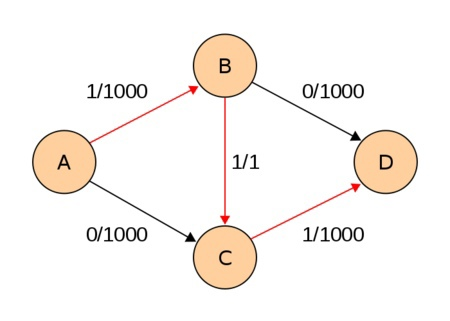
\includegraphics[width=\linewidth]{images/72-85_ff_example1.jpg}}
\end{minipage}
\hfill
\hspace{-4ex} \begin{minipage}[h]{0.3\linewidth}
\center{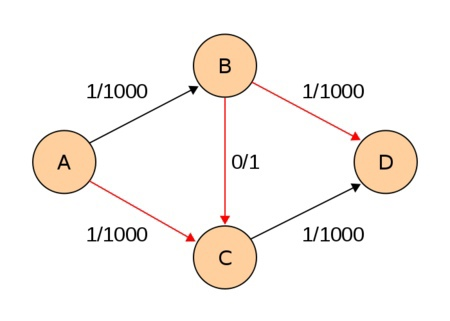
\includegraphics[width=\linewidth]{images/72-85_ff_example2.jpg}}
\end{minipage}
\hfill
\hspace{-4ex} \begin{minipage}[h]{0.3\linewidth}
\center{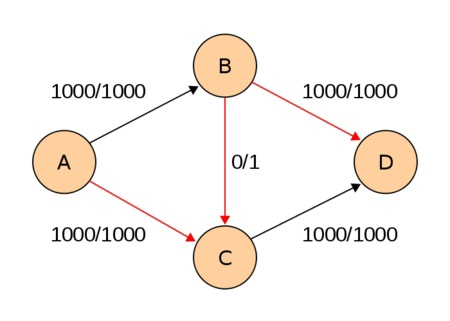
\includegraphics[width=\linewidth]{images/72-85_ff_example3.jpg}}
\end{minipage}
\end{figure}
\par \textbf{Асимптотика:} $O(ans \cdot (n+m))$ - размер ответа (может быть что на каждой итерации проталкиваем по единице потока) умноженный на асимптотику поиска пути (DFS)

\setcounter{section}{76}
\section{Алгоритм Эдмондса—Карпа. Корректность.}
\par \textbf{Алгоритм Эдмондса-Карпа:} На каждой итерации алгоритма Форда-Фалкерсона находим путь, кратчайший по количеству ребер в нем.
\par \textbf{Корректность:} очевидно следует из теоремы Форда-Фалкерсона (см. билет 75)

\setcounter{section}{77}
\section{Лемма о возрастании $dist(s, v)$ между последовательными итерациями алгоритма Эдмондса-Карпа.}
\par \textbf{Лемма:} Пусть $f$ и $f'$ два последовательных потока в алгоритме. Пусть $d(v)=dist(s,v)$ в $G_f$, $d'(v)=dist(s,v)$ в $G_{f'}$. Тогда $\forall v \in V \hookrightarrow d'(v) \geq d(v)$
\par $\blacktriangle$ Если $v=s$, то $d'(v)=0=d(v)$ и все доказано.
\par Пусть $v \neq s$. Среди всех $v$ таких что выполнено $d'(v)<d(v)$ найдём $v$ такую что $d'(v)$ минимально.
\par Пусть $u$ - предпоследняя вершина на кратчайшем пути из $s$ в $v$ в $G_{f'}$. Тогда $d'(u)+1=d'(v) \: (1)\Rightarrow d'(u) < d'(v) \Rightarrow$ так как $d'(v)$ - минимальное такое что $d'(v)<d(v)$, а $d'(u)<d'(v)$, то $d'(u) \geq d(u) \: (2)$.
\par Как ребро $(u,v)$ оказалось в $G_{f'}$? Рассмотрим 2 случая \begin{enumerate}
    \item $(u,v)$ было в $G_f$. Тогда $d(v)\leq d(u)+1$ (кратчайший путь до $v$ не больше чем путь до $v$ через $u$) $\stackrel{(2)}{\leq} d'(u)+1 \stackrel{(1)}{=} d'(v)$ - противоречие с выбором $v$.
    \item $(u,v)$ появилось только в $G_{f'}$. Значит оно появилось как обратное к ребру $(v,u)$, по которому был пропущен поток, то есть оно лежало на кратчайшем пути из $s$ в $t$ в $G_f$ $\Rightarrow d(v)+1=d(u)\stackrel{(2)}{\leq} d'(u)\stackrel{(1)}{=} d'(v)-1 \Rightarrow d(v)+2\leq d'(v) \Rightarrow d'(v)>d(v)$ - противоречие с выбором $v$
\end{enumerate}
\par Так как в обоих случаях получили противоречие, то таких $v$ не существует, а значит $\forall v \in V \hookrightarrow d'(v) \geq d(v) \: \blacksquare$

\setcounter{section}{78}
\section{Лемма о числе насыщений ребра в алгоритме Эдмондса-Карпа. Асимптотика этого алгоритма.}
\par \textbf{Лемма:} Говорим, что ребро насыщается, если $f(u,v)$ становится равным $c(u,v)$. Тогда каждое ребро насыщается $O(V)$ раз.
\par $\blacktriangle$ Пусть ребро $(u,v)$ насытилось (назовем этот момент 1). Чтобы оно насытилось еще раз, его надо «разнасытить», то есть кратчайший путь из $s$ в $t$ должен проходить через $(v,u)$ (обозначим этот момент как 2)
\par Пусть $d$ - кратчайшее расстояние в момент 1, а $d'$ - в момент 2. Тогда $d(v)=d(u)+1$ (так как в момент 1 $(u,v)$ лежало на кратчайшем пути из $s$ в $t$), $d'(v) \geq d(v)$ (по прошлой лемме), $d'(u)=d'(v)+1$ (так как ребро $(v,u)$ в момент 2 лежало на кратчайшем пути из $s$ в $t$). Получаем $d'(u)=d'(v)+1 \geq d(v)+1=d(u)+2 \Rightarrow$ чтобы $(u,v)$ разнасытилось, $d(u)$ должно вырасти хотя бы на 2, $d(u) \leq V - 1 \Rightarrow$ это происходит $\leq \frac{V}{2}$ раз $\blacksquare$
\par \textbf{Асимптотика:} $O(VE^2)$ - всего $O(VE)$ итераций (ребер $E$, каждое насыщается $O(V)$ раз) на каждой итерации ищем кратчайший путь через $BFS$ ($O(E)$)
\setcounter{section}{79}
\section{Задача о разбиении коллектива на две группы с минимизацией суммарного недовольства.}
\par \textbf{Формулировка задачи:} Есть $n$ людей, нужно разбить их на 2 группы: занимающихся математикой и программированием. Каждый из них имеет некоторое недовольство к математике ($a_i$) и к программированию ($b_i$). Также между некоторыми из них есть дружеские связи, при разрыве которых суммарное недовольство увеличивается (на $c_{ij}$). Необходимо найти такое разбиение, чтобы суммарное недовольство было минимальным.
\par \textbf{Решение:} Создадим по одной вершине для каждого человека и две вершины $s$ и $t$. Для кадого $i$ \begin{enumerate}
    \item Проведем ребро $(s,i)$ с capacity $a_i$
    \item Проведем ребро $(i,t)$ с capacity $b_i$
    \item Для каждого друга $j$ проведем два ребра $(i,j)$ и $(j, i)$ с capacity $c_{ij}$
\end{enumerate}
\par Искомому разбиению с минимальным недовольством будет соответствовать минимальный разрез в построенном графе ($S$ - программисты, $T$ - математики)
\begin{figure}[h]
\center{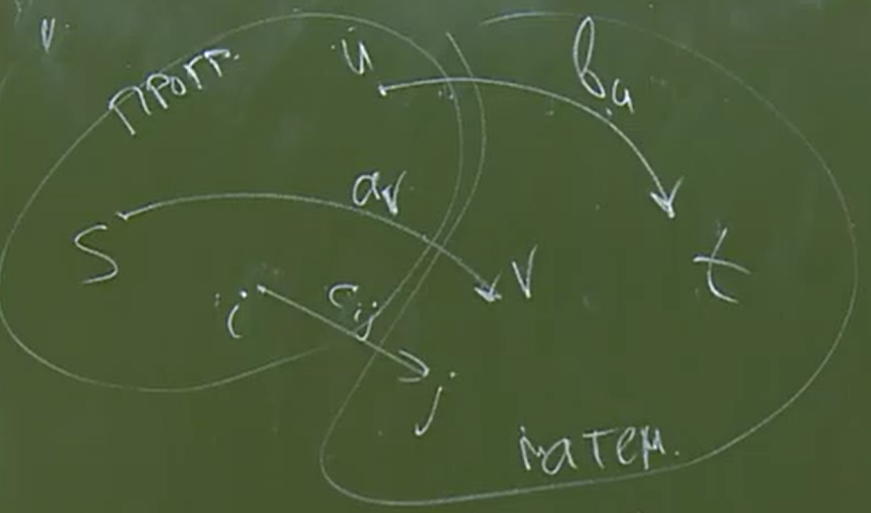
\includegraphics[scale=0.5]{images/72-85_nedovolstvo.png}}
\end{figure}
\par Из картинки видно почему это правда: для каждой вершины будет учтено недовольство своей текущей профессией, а также разорванные дружбы (будут учтены только один раз по определению величины разреза).
\\

\setcounter{section}{80}
\section{Алгоритм Эдмондса-Карпа с масштабированием, асимптотика.}
\par Пусть $C$ - верхнее ограничение на все capacity. Перебираем $k=\lceil \log_2 C \rceil \ldots 0$, на $k$-ом шаге алгоритма рассматриваем сеть с $c'(e)=\lfloor \frac{c_f(e)}{2^k} \rfloor \cdot 2^k$, например
 \begin{itemize}
    \item[]$c_f(e)<2^k \Rightarrow c'(e)=0$
    \item[] $2^k\leq c_f(e)<2^{k+1}\Rightarrow c'(e)=2^k$
\end{itemize}
\par \textbf{Алгоритм:} Перебираем  $k=\lceil \log_2 C \rceil \ldots 0$, находим и проталкиваем максимальный поток в сети $c'(e)$ (находим его Эдмондсом-Карпом, может быть проталкиваем по нескольким путям если получится).
\par \textbf{Асимптотика:} $O(E^2 \log C)$
\par $\blacktriangle$ Понятно, что $\log C$ - это количество итераций. Покажем, что на каждой итерации мы находим $O(E)$ путей (из $O(E)$ на поиск одного пути как раз получится искомая асимптотика.
\par Пусть после рассмотрения $k$ пропустили поток $F_k$. Рассмотрим разрез: в одной части все вершины достижимые из $S$ по ребрам $\geq 2^k$, в другой - остальные. Тогда величина разреза $\leq 2^kE$ (все ребра между частями $<2^k$) следовательно $F-F_k \leq 2^k E$, так как оставшийся поток не превосходит разреза.
\par Рассмотрим $k$-ый шаг. Заметим, что каждый раз когда мы увеличиваем поток, он увеличивается хотя бы на $2^k$. Так как наш поток отличается от максимального на $\leq 2^k E$, то увеличить поток мы сможем $O(E)$ раз. Итог: на каждом шаге делаем DFS $O(E)$ раз. Таким образом, получаем асимптотику $O(E^2 \log C)$ $\blacksquare$

\setcounter{section}{81}
\section{Определение слоистой сети, блокирующего потока. Алгоритм Диница, доказательство корректности.}
\par \textbf{Определение:} $G$ - сеть, $V_i=\{v \: | \: dist(s,v)=i\}$ - слои. Тогда \textit{слоистая сеть} построенная по $G$ - сеть, в которой оставлены только ребра из меньших слоев в большие (ребра из больших слоев в меньшие и внутри слоев игнорируются)
\par \textbf{Определение:} Пусть $G$ - сеть. Тогда \textit{блокирующим потоком} в ней называется такой поток, который нельзя увеличить без введения обратных ребер.
\par \textbf{Алгоритм Диница:} Пока из $s$ в $t$ есть путь в $G_f$ строим слоистую сеть и ищем в ней блокирующий поток.
\par \textbf{Корректность:} остановимся только когда нет пути из $s$ в $t$ в остаточной сети $\Rightarrow$ алгоритм корректен по теореме Форда-Фалкерсона

\setcounter{section}{82}
\section{Реализация алгоритма Диница. Асимптотика.}
\par Слоистая сеть строится просто через 1 BFS (запускаем и оставляем только те ребра, которые идут из расстояния $i$ в $i+1$)
\par Как же искать блокирующий поток? Рассмотрим одну вершину $v$ каждое ребро выходящее из нее имеет смысл рассматривать только один раз: если мы нашли путь, то просто проталктваем туда поток, а если не нашли, то в будущем мы уже и не найдем, поэтому считаем его "неинтересным". Введем $ptr[v]$ - номер первого интересного ребра исходящего из $v$.
\lstinputlisting[language=C++,
emph={int,char,double,float,unsigned},
emphstyle={\color{blue}}
]{code/72-85_dfs.cpp}

\textbf{Весь алгоритм Диница:}
\lstinputlisting[language=C++,
emph={int,char,double,float,unsigned},
emphstyle={\color{blue}}
]{code/72-85_diniz.cpp}

\par \textbf{Асимптотика:} $O(V^2 E)$
\par $\blacktriangle$ Рассмотрим асимптотику операции $dfs(s, \infty)$. Если за время ее выполнения указатели интересных ребер сместились на $k$, то ее асимптотика - это $O(V+k)$. Действительно, все что мы делаем - это проходим по одному пути (максимальной длины $V$) и переключаем $k$ указателей.
\par Тогда одна итерация алгоритма Диница работает за $O(V\cdot \text{(количество найденных путей)}+\text{(суммарное изменение всех указателей)})$. Количество найденных путей не превосходит $E$, так как каждый новый путь насыщает хотя бы одно ребро. Суммарное изменение всех указателей также не превосходит $E$ (так как всего ребер $E$) $\Rightarrow$ асимптотика одной итерации алгоритма Диница равна $O(VE)$.
\par Покажем, что после каждой итерации $dist'(s,t)>dist(s,t)$. После пропускания блокирующего потока в остаточной сети могли добавиться только ребра из $i$-го слоя в $i-1$-й, (так как поток пускаем только по ребрам из $i$-го в $i+1$-й). Очевидно, что такие ребра не могут сократить расстояние между $s$ и $t$ лежащими в $0$ и $l$-ом слоях. Пусть $dist(s,t)$ остался таким же. Заметим, что у нас всего $dist(s,t)+1$ слоев и есть ребра либо вперед на один слой, либо назад на один слой. Очевидно, что чтобы получился путь длины $dist(s,t)$ мы можем прыгать только вперед на 1 слой. Следовательно, этот путь полностью лежит в нашей слоистой сети, а значит мы можем пустить по нему поток - противоречие с тем, что нашли блокирующий поток
\par Таким образом, так как расстояние между $s$ и $t$ постоянно растет в алгоритме Диница всего $O(V)$ итераций $\Rightarrow$ общая асимптотика равна $O(V^2 E) \: \blacksquare$
\setcounter{section}{83}
\section{Первая теорема Карзанова о числе итераций алгоритма Диница.}
\par \textbf{Обозначения:} для любой вершины $v$ отличной от $s$ и $t$ введем следующие величины:
$$C_{in}(v)=\sum_{u \in V}c(u,v); \: C_{out}(v)=\sum_{w \in V} c(v, w) \text{ - входящая и исходящая capacity}$$
$$p(v)=\min(C_{in}(v), C_{out}(v)) \text{ - потенциал вершины}$$
$$P=\sum_{v \in V \setminus \{s, t\}} p(v) \text{ - потенциал сети}$$
\par \textbf{Замечание:} Через $v$ может протекать не больше чем $p(v)$ потока, так как потенциал вершины - это минимум из входящей и исходящей capacity и выполнен закон сохранения потока.
\par \textbf{Лемма:} Пусть $L=dist(s,t), F$ - максимальный поток. Тогда $L \leq \frac{P}{F}+1$
\par $\blacktriangle$ Так как $L=dist(s,t)$ в слоистой сети есть $L+1$ слой включая слои содержащие $s$ и $t$ (слоев без $s$ и $t$ - $L-1$). Обозначим $P_i=\sum_{v \in V_i} p(v)$. \par Через $V_i$ протекает $\leq P_i$ потока, так как $P_i$ - это сумма потенциалов всех вершин в слое $\Rightarrow F \leq P_i \Rightarrow  (L-1)F \leq P_1+\ldots +P_{l-1} \leq P \Rightarrow L \leq \frac{P}{F}+1 \: \blacksquare$
\par \textbf{Лемма:} $P$ не изменяется при проталкиванях потока при переходе к остаточной сети.
\begin{figure}[h]
\hspace{-4ex} \begin{minipage}[h]{0.3\linewidth}

\center{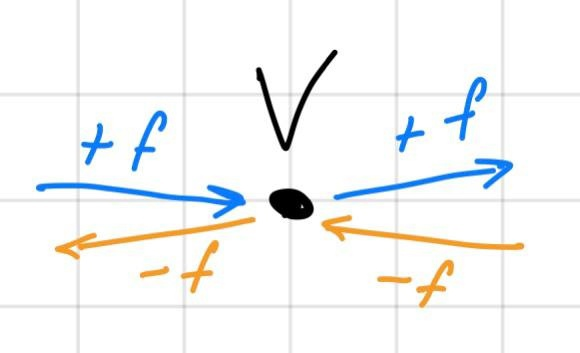
\includegraphics[scale=0.25]{images/72-85_flow.jpg}}
\end{minipage}
\hfill
\hspace{-4ex} \begin{minipage}[h]{0.7\linewidth}
\par $\blacktriangle$ Пусть $v$ лежит на пути, по которому протолкнули поток $f$ в остаточной сети. Тогда capacity ребер лежащих на этом пути уменьшилась на $f$, а обратных - увеличилась на $f$. После изображения такого изменения на картинке вижно, что $C_{in}$ и $C_{out}$ не поменялись, а значит и $p(v)$ не поменялся $\Rightarrow$ потенциал всей сети также не поменялся $\blacksquare$
\end{minipage}
\end{figure}
\par \textbf{Теорема (первая теорема Карзанова):} Число итераций алгоритма Диница равно $O(\sqrt{P}$).
\par $\blacktriangle$ Сделаем $\sqrt{P}$ итераций алгоритма Диница. Тогда $dist(s,t)=l_{new} \geq \sqrt{P}$ (так как доказали, что на каждой итерации $dist(s,t)$ увеличивается в билете 83). По лемме $\sqrt{P} \leq l_{new} \leq \frac{P}{F_{\text{ост}}}+1 \Rightarrow \sqrt{P}-1 \leq \frac{P}{F_{\text{ост}}} \Rightarrow F_{\text{ост}} \leq \frac{P}{\sqrt{P}-1}=O(\sqrt{P})$. Так как осталось пропустить $O(\sqrt{P})$ потока, то осталось найти $O(\sqrt{P})$ путей $\Rightarrow$ осталось $O(\sqrt{P})$ итераций. Так как до этого мы сделали ровно $\sqrt{P}$ итераций, то всего у нас тоже получается $O(\sqrt{P})$ итераций $\blacksquare$
\par \textbf{Теорема (вторая теорема Карзанова):} Число итераций алгоритма Диница равно $O(C^{1/3} V^{2/3})$, где $C$ - ограничение сверху на все capacity (нет в программе, для общего развития).
\\

\setcounter{section}{84}
\section{Эффективность алгоритма  Диница в единичных сетях.}
\par \textbf{Определение:} \textit{Единичная сеть} - сеть, в которой capacity принимают только значения 0 и 1
\par \textbf{Замечание 1:} В единичной сети $P \leq O(E)$
\par $\blacktriangle$ Так как сеть единичная, то $C_{in}(v)=deg_{in}(v); \: C_{out}(v)=deg_{out}(v)$, где $deg_{in}, \: deg_{out}$ - входящая и исходящая степени вершины соответственно (то есть количество ребер входящих и выходящих из вершины). Тогда по определению $$p(v)=\min(deg_{in}(v), deg_{out}(v)) \leq deg_{in}(v) + deg_{out}(v)$$Откуда получаем, что $$P = \sum_{v \in V \setminus \{ s, t\}} p(v) \leq \sum_{v \in V} deg_{in}(v) + \sum_{v \in V} deg_{out}(v) = 2E \: \blacksquare$$
\par \textbf{Замечание 2:} В единичной сети одна итерация алгоритма Диница работает за $O(E)$ так как за все $dfs$ы ребро рассматривается максимум 1 раз (либо протолкнем по нему поток, либо выкинем из рассмотрения как неинтересное).
\par \textbf{Вывод:} В единичной сети алгоритм Диница работает за $O(E\sqrt{E})$